% Created by tikzDevice version 0.12.5 on 2023-10-23 22:31:07
% !TEX encoding = UTF-8 Unicode
\definecolor{color1}{HTML}{CC9966}
\definecolor{color2}{HTML}{99CCFF}
\definecolor{viridis0}{RGB}{255, 255, 255}
\definecolor{viridis1}{RGB}{253, 231, 37}
\definecolor{viridis2}{RGB}{181, 222, 43}
\definecolor{viridis3}{RGB}{110, 206, 88}
\definecolor{viridis4}{RGB}{53, 183, 121}
\definecolor{viridis5}{RGB}{31, 158, 137}
\definecolor{viridis6}{RGB}{38, 130, 142}
\definecolor{viridis7}{RGB}{49, 104, 142}
\definecolor{viridis8}{RGB}{62, 73, 137}
\definecolor{viridis9}{RGB}{72, 40, 120}
\definecolor{viridis10}{RGB}{68, 1, 84}
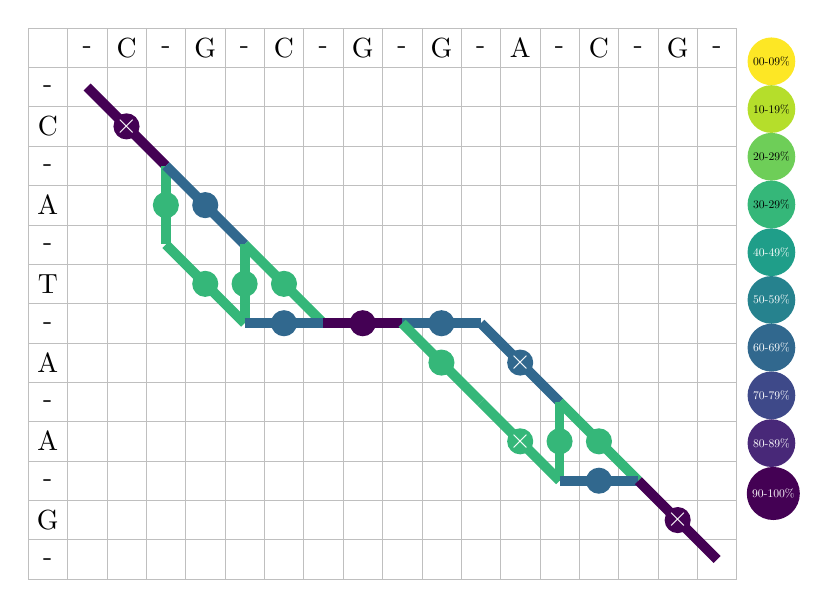
\begin{tikzpicture}[dot/.style={circle, minimum size=2.5mm}]
\draw[very thin, color = gray!50, step = 0.5] (0,0) grid (9, 7);
\node at (0.25,6.25) {-};
\node at (0.25,5.75) {C};
\node at (0.25,5.25) {-};
\node at (0.25,4.75) {A};
\node at (0.25,4.25) {-};
\node at (0.25,3.75) {T};
\node at (0.25,3.25) {-};
\node at (0.25,2.75) {A};
\node at (0.25,2.25) {-};
\node at (0.25,1.75) {A};
\node at (0.25,1.25) {-};
\node at (0.25,0.75) {G};
\node at (0.25,0.25) {-};
\node at (0.75,6.75) {-};
\node at (1.25,6.75) {C};
\node at (1.75,6.75) {-};
\node at (2.25,6.75) {G};
\node at (2.75,6.75) {-};
\node at (3.25,6.75) {C};
\node at (3.75,6.75) {-};
\node at (4.25,6.75) {G};
\node at (4.75,6.75) {-};
\node at (5.25,6.75) {G};
\node at (5.75,6.75) {-};
\node at (6.25,6.75) {A};
\node at (6.75,6.75) {-};
\node at (7.25,6.75) {C};
\node at (7.75,6.75) {-};
\node at (8.25,6.75) {G};
\node at (8.75,6.75) {-};
\draw[line width=1.25mm,viridis10](0.75,6.25)--(1.25,5.75);
\draw[line width=1.25mm,viridis10](1.25,5.75)--(1.75,5.25);
\node[circle, fill=viridis10] at (1.25, 5.75){};
\node[white] at (1.25, 5.75) {$\mathlarger{\mathlarger{\bm{\times}}}$};
\draw[line width=1.25mm,viridis4](1.75,5.25)--(1.75,4.75);
\draw[line width=1.25mm,viridis7](1.75,5.25)--(2.25,4.75);
\draw[line width=1.25mm,viridis4](1.75,4.75)--(1.75,4.25);
\node[circle, fill=viridis4] at (1.75, 4.75){};
\draw[line width=1.25mm,viridis7](2.25,4.75)--(2.75,4.25);
\node[circle, fill=viridis7] at (2.25, 4.75){};
\draw[line width=1.25mm,viridis4](1.75,4.25)--(2.25,3.75);
\draw[line width=1.25mm,viridis4](2.75,4.25)--(2.75,3.75);
\draw[line width=1.25mm,viridis4](2.75,4.25)--(3.25,3.75);
\draw[line width=1.25mm,viridis4](2.25,3.75)--(2.75,3.25);
\node[circle, fill=viridis4] at (2.25, 3.75){};
\draw[line width=1.25mm,viridis4](2.75,3.75)--(2.75,3.25);
\node[circle, fill=viridis4] at (2.75, 3.75){};
\draw[line width=1.25mm,viridis4](3.25,3.75)--(3.75,3.25);
\node[circle, fill=viridis4] at (3.25, 3.75){};
\draw[line width=1.25mm,viridis7](2.75,3.25)--(3.25,3.25);
\draw[line width=1.25mm,viridis7](3.25,3.25)--(3.75,3.25);
\node[circle, fill=viridis7] at (3.25, 3.25){};
\draw[line width=1.25mm,viridis10](3.75,3.25)--(4.25,3.25);
\draw[line width=1.25mm,viridis10](4.25,3.25)--(4.75,3.25);
\node[circle, fill=viridis10] at (4.25, 3.25){};
\draw[line width=1.25mm,viridis7](4.75,3.25)--(5.25,3.25);
\draw[line width=1.25mm,viridis4](4.75,3.25)--(5.25,2.75);
\draw[line width=1.25mm,viridis7](5.25,3.25)--(5.75,3.25);
\node[circle, fill=viridis7] at (5.25, 3.25){};
\draw[line width=1.25mm,viridis7](5.75,3.25)--(6.25,2.75);
\draw[line width=1.25mm,viridis4](5.25,2.75)--(5.75,2.25);
\node[circle, fill=viridis4] at (5.25, 2.75){};
\draw[line width=1.25mm,viridis7](6.25,2.75)--(6.75,2.25);
\node[circle, fill=viridis7] at (6.25, 2.75){};
\node[white] at (6.25, 2.75) {$\mathlarger{\mathlarger{\bm{\times}}}$};
\draw[line width=1.25mm,viridis4](5.75,2.25)--(6.25,1.75);
\draw[line width=1.25mm,viridis4](6.75,2.25)--(6.75,1.75);
\draw[line width=1.25mm,viridis4](6.75,2.25)--(7.25,1.75);
\draw[line width=1.25mm,viridis4](6.25,1.75)--(6.75,1.25);
\node[circle, fill=viridis4] at (6.25, 1.75){};
\node[white] at (6.25, 1.75) {$\mathlarger{\mathlarger{\bm{\times}}}$};
\draw[line width=1.25mm,viridis4](6.75,1.75)--(6.75,1.25);
\node[circle, fill=viridis4] at (6.75, 1.75){};
\draw[line width=1.25mm,viridis4](7.25,1.75)--(7.75,1.25);
\node[circle, fill=viridis4] at (7.25, 1.75){};
\draw[line width=1.25mm,viridis7](6.75,1.25)--(7.25,1.25);
\draw[line width=1.25mm,viridis7](7.25,1.25)--(7.75,1.25);
\node[circle, fill=viridis7] at (7.25, 1.25){};
\draw[line width=1.25mm,viridis10](7.75,1.25)--(8.25,0.75);
\draw[line width=1.25mm,viridis10](8.25,0.75)--(8.75,0.25);
\node[circle, fill=viridis10] at (8.25, 0.75){};
\node[white] at (8.25, 0.75) {$\mathlarger{\mathlarger{\bm{\times}}}$};
\matrix [draw, below right, draw=none] at (current bounding box.north east) {
        % \node[circle, fill=viridis0, scale=0.75] {0\%}; \\
        \node[circle, fill=viridis1, scale=0.42] {00-09\%}; \\
        \node[circle, fill=viridis2, scale=0.42] {10-19\%}; \\
        \node[circle, fill=viridis3, scale=0.42] {20-29\%}; \\
        \node[circle, fill=viridis4, scale=0.42] {30-29\%}; \\
        \node[circle, fill=viridis5, scale=0.42] {\textcolor{white}{40-49\%}}; \\
        \node[circle, fill=viridis6, scale=0.42] {\textcolor{white}{50-59\%}}; \\
        \node[circle, fill=viridis7, scale=0.42] {\textcolor{white}{60-69\%}}; \\
        \node[circle, fill=viridis8, scale=0.42] {\textcolor{white}{70-79\%}}; \\
        \node[circle, fill=viridis9, scale=0.42] {\textcolor{white}{80-89\%}}; \\
        \node[circle, fill=viridis10, scale=0.42] {\textcolor{white}{90-100\%}}; \\
    };
\end{tikzpicture}
